% The MIT License

% Copyright 2023 Shunsuke KIMURA

% Permission is hereby granted, free of charge, to any person obtaining a copy of this software and associated documentation files (the “Software”), to deal in the Software without restriction, including without limitation the rights to use, copy, modify, merge, publish, distribute, sublicense, and/or sell copies of the Software, and to permit persons to whom the Software is furnished to do so, subject to the following conditions:

% The above copyright notice and this permission notice shall be included in all copies or substantial portions of the Software.

% THE SOFTWARE IS PROVIDED “AS IS”, WITHOUT WARRANTY OF ANY KIND, EXPRESS OR IMPLIED, INCLUDING BUT NOT LIMITED TO THE WARRANTIES OF MERCHANTABILITY, FITNESS FOR A PARTICULAR PURPOSE AND NONINFRINGEMENT. IN NO EVENT SHALL THE AUTHORS OR COPYRIGHT HOLDERS BE LIABLE FOR ANY CLAIM, DAMAGES OR OTHER LIABILITY, WHETHER IN AN ACTION OF CONTRACT, TORT OR OTHERWISE, ARISING FROM, OUT OF OR IN CONNECTION WITH THE SOFTWARE OR THE USE OR OTHER DEALINGS IN THE SOFTWARE.

\documentclass[aspectratio=169,dvipdfmx,cjk]{beamer} 
\usetheme{Madrid}
\setbeamertemplate{navigation symbols}{}
\setbeamertemplate{footline}[frame number]
\usepackage{pxjahyper}
\usepackage{cite}
\usepackage{minijs}
\usepackage{listings}
\usepackage{graphicx}
\usepackage{svg}
\usepackage{xcolor}
\hypersetup{
  colorlinks=false,
  citebordercolor=green,
  linkbordercolor=red,
  urlbordercolor=cyan,
}
\lstdefinestyle{command}{
  backgroundcolor=\color{lightgray},
  basicstyle=\ttfamily\color{black},
  stringstyle={\small\ttfamily},
  keywordstyle=\color{blue},
  commentstyle=\color{gray},
  showstringspaces=false,
  frame=single,
  rulecolor=\color{lightgray},
  breaklines=true,
  numbers=left,
}
\newcommand{\cmdline}[1]{
    \colorbox{lightgray}{\lstinline[style=command]{#1}}
}
\newcommand{\blue}[1]{ {\color{blue} #1} }

\title{platex-vscode-template の使い方}
\author{Shunsuke Kimura}
\date{\today}

\begin{document}

\begin{frame}
  \titlepage
\end{frame}

\begin{frame}{はじめに}
  \begin{block}{概要}
    Windows を使う初学者を対象に \href{https://github.com/kimushun1101/platex-vscode-template}{https://github.com/kimushun1101/platex-vscode-template} で説明している内容のスクリーンショットを並べる.\\
    ここではとりあえず方法だけ紹介するので,気になる方は各自キーワードで検索してください.
  \end{block}
  \begin{block}{この資料でできること}
    \begin{enumerate}
      \item Windows 上にコンパイル速度が早い \LaTeX 環境の構築
      \item \LaTeX 文書作成のワークフローの習得
      \item GitHub を用いたバージョン管理および共有作業
    \end{enumerate}
  \end{block}
  \begin{tiny}
    パスワード漏洩防止や権限の適切な設定などは各人・各組織でご管理ください.
    この資料のソースコードは MIT License としています.
  \end{tiny}
\end{frame}

\begin{frame}{目次}
  \tableofcontents
\end{frame}

\begin{frame}{全体構成}
  \centering
  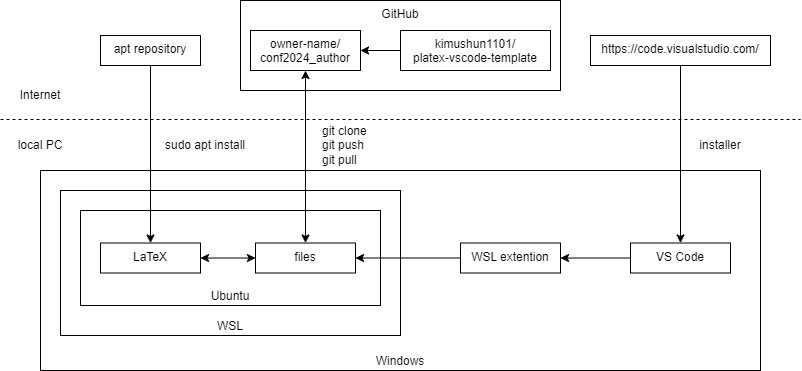
\includegraphics[width=0.9\linewidth]{fig/structure.png}
  \begin{tiny}
    \rightline{owner-name は適宜ご自身のユーザ名や組織名に置き換えてお考えください(後述).}
  \end{tiny}
  多少複雑ですが,他ソースコードの編集や管理などにも流用できる技術で構成しております.
\end{frame}


\section{(初回のみ) 環境構築}

\subsection{WSL のインストール}
\begin{frame}{\insertsection \thesubsection: \insertsubsection}
  公式ページ\cite{WSL}に従う
  \begin{enumerate}
    \item PowerShell を\blue{管理者モード}で実行.
    \item \cmdline{wsl --install} コマンドを入力.
    \item PCを再起動.
  \end{enumerate}
  \begin{columns}
    \begin{column}{0.33\textwidth}
        
\includegraphics[width=1.0\linewidth]{fig/robot.png}
    \end{column}
    \begin{column}{0.33\textwidth}
      
\includegraphics[width=1.0\linewidth]{fig/robot.png}
    \end{column}
    \begin{column}{0.33\textwidth}
      
\includegraphics[width=1.0\linewidth]{fig/robot.png}
    \end{column}
  \end{columns}
\end{frame}

\subsection{Ubuntu のインストール}
\begin{frame}{\insertsection \thesubsection: \insertsubsection}
  公式ページ\cite{WSL}に従う
  \begin{enumerate}
    \item PowerShell を実行.今回は管理者モードでなくてよい.
    \item \cmdline{wsl --install Ubuntu} コマンドを入力.
    \item ユーザ名とパスワードを設定し,ログインできたら画面を閉じる.
  \end{enumerate}
  \begin{columns}
    \begin{column}{0.33\textwidth}
        
\includegraphics[width=1.0\linewidth]{fig/robot.png}
    \end{column}
    \begin{column}{0.33\textwidth}
      
\includegraphics[width=1.0\linewidth]{fig/robot.png}
    \end{column}
    \begin{column}{0.33\textwidth}
      
\includegraphics[width=1.0\linewidth]{fig/robot.png}
    \end{column}
  \end{columns}
\end{frame}

\subsection{\LaTeX (とGit)のインストール}
\begin{frame}{\insertsection \thesubsection: \insertsubsection}
  \begin{enumerate}
    \item Ubuntu を実行.
    \item 以降,コマンド入力は PowerShell ではなく Ubuntu の画面に対して行う.\\ \cmdline{sudo apt update && sudo apt install texlive-full git -y} コマンドを入力.
  \end{enumerate}
\end{frame}

\subsection{VS Code のインストール}
\begin{frame}{\insertsection \thesubsection: \insertsubsection}
  \begin{enumerate}
    \item ブラウザで\href{https://code.visualstudio.com/}{https://code.visualstudio.com/}を開く.
    \item \beamerbutton{Download for Windows} をクリックしてインストーラーをダウンロード.その後それを実行.
    \item インストール中に [追加タスクの選択] が求められたときは、[PATH への追加] オプションがオンになっていることを確認.
    \item インストール後に VS Code を実行して \beamerbutton{Ctrl + P} で現れるテキストボックスに \cmdline{ext install ms-vscode-remote.remote-wsl} を入力して WSL Extension を install.
  \end{enumerate}
  \begin{columns}
    \begin{column}{0.33\textwidth}
        
\includegraphics[width=1.0\linewidth]{fig/robot.png}
        右クリック
    \end{column}
    \begin{column}{0.33\textwidth}
      
\includegraphics[width=1.0\linewidth]{fig/robot.png}
    \end{column}
    \begin{column}{0.33\textwidth}
      
\includegraphics[width=1.0\linewidth]{fig/robot.png}
    \end{column}
  \end{columns}
\end{frame}

\subsection{GitHub アカウントの作成}
\begin{frame}{\insertsection \thesubsection: \insertsubsection}
  \begin{enumerate}
    \item ブラウザで \href{https://github.com/}{https://github.com/} にアクセスして,\beamerbutton{Sign up for GitHub} から,ユーザ名やEメールアドレス,パスワードなどを設定\cite{GitHubAccount}.以降ログインした状態とする.
    \item Ubuntu に\cmdline{ssh-keygen -t ed25519 -C "your_email@example.com"} コマンドを\blue{自身のメールアドレスに置き換えて}入力.パスフレーズを設定しない場合には何も入力せずEnterを3回くらいすればよい.気になる人は各自で調べてください\cite{GitHubSSH}.
    \item \cmdline{cat ~/.ssh/id_ed25519.pub} コマンドで出力された文字列をコピー\cite{GitHubAccount}.
    \item ブラウザで\href{https://github.com/settings/ssh}{https://github.com/settings/ssh} にアクセスして,\beamerbutton{New SSH key} からコピーした文字列を Key にペーストして登録\cite{GitHubAccount}.Title はこの操作を行っているPCを指す文字列,Key type はAuthentication Key のままでOK.
  \end{enumerate}
  \begin{columns}
    \begin{column}{0.33\textwidth}
        
\includegraphics[width=1.0\linewidth]{fig/robot.png}
    \end{column}
    \begin{column}{0.33\textwidth}
      
\includegraphics[width=1.0\linewidth]{fig/robot.png}
    \end{column}
    \begin{column}{0.33\textwidth}
      
\includegraphics[width=1.0\linewidth]{fig/robot.png}
    \end{column}
  \end{columns}
\end{frame}

\section{文書作成}
\subsection{リモート Repository の作成}
\begin{frame}{\insertsection \thesubsection: \insertsubsection}
  \begin{enumerate}
    \item \href{https://github.com/kimushun1101/platex-vscode-template}{https://github.com/kimushun1101/platex-vscode-template} にアクセス.
    \item \beamerbutton{Use this template} から \beamerbutton{create a new repository} を選択
    \item 推奨設定(あとから変更も可能)
    \begin{itemize}
      \item 共有したい場合には Owner を組織アカウントに変更.
      \item Repository name は,ディレクトリ名(フォルダ名)になります.投稿先や筆頭著者名,タイトル名の一部など識別できるものにしましょう.\\
      以下,例として \cmdline{conf2024_author} としたとして進める.
      \item Private Repository にチェックを入れる.
    \end{itemize}
  \end{enumerate}
\end{frame}

\subsection{ローカル Workspace の設定}
\begin{frame}{\insertsection \thesubsection: \insertsubsection}
  \begin{enumerate}
    \item 前スライドで作成したRepositoryのページを開く.
    \href{https://github.com/}{https://github.com/} から探せる.
    \item \beamerbutton{$< >$ Code▼} から \beamerbutton{SSH} タブを選択,\beamerbutton{□が2つ重なったような記号} をクリックして URL をコピー.
    \item Ubuntu に \cmdline{git clone URL} コマンドを\blue{コピーしたURLに置き換えて}入力.
    \item Ubuntu に \cmdline{code conf2024_author} コマンドを\blue{自身のrepository名に置き換えて}入力することで,VS Code を起動する.
    \begin{itemize}
      \item \cmdline{ls} コマンドをすると現在存在するディレクトリを確認できる.興味があれば「Unix コマンド」で調べてみるとよい.移動や削除など,よりいろいろな操作ができるようになるだろう.
      \item たとえば \cmdline{code conf[Tab]} という感じで,途中まで入力してTab キーで補完もできる.
    \end{itemize}
  \end{enumerate}
\end{frame}

\subsection{(初回のみ) VS Code の設定}
\begin{frame}{\insertsection \thesubsection: \insertsubsection}
  \begin{enumerate}
    \item VS Code の Extensions を開く.ショートカットは \beamerbutton{Ctrl + Shif + X}.
    \item 検索ボックス右の Filter Extensions をクリックして,\beamerbutton{recommended} を選択して出てきたものをすべてインストールする.
  \end{enumerate}
\end{frame}

\subsection{編集作業}
\begin{frame}{\insertsection \thesubsection: \insertsubsection}
  \begin{enumerate}
    \item sample.tex を開く
    \item \beamerbutton{Ctrl + Alt + B} でビルド.ファイル保存時もオートビルドされる.
    \item \beamerbutton{Ctrl + Alt + V} でコンパイル済みPDFを表示.
  \end{enumerate}
  その他のショートカットは以下の通り.\\
  \vspace{10mm}
  \centering
  \begin{tabular}{ll} \hline
    ショートカット & 機能 \\
    \hline
    \beamerbutton{Ctrl + Alt + J} & PDF の該当の場所にジャンプ \\
    PDF を \beamerbutton{Ctrl} + クリック & .tex の該当の行にジャンプ \\
    \beamerbutton{Ctrl + Alt + M} & 数式プレビューの表示 \\
    \beamerbutton{Ctrl + J} (PROBLEMS タブ) & エラーやワーニングの確認 \\
    \beamerbutton{F8} & エラーやワーニングへジャンプ \\
    \hline
  \end{tabular}
\end{frame}

\subsection{バージョンの保存}
\begin{frame}{\insertsection \thesubsection: \insertsubsection}
  \begin{enumerate}
    \item VS Code で Source Control を開く.ショートカットキーは \beamerbutton{Ctrl + Shift + G}.
    \item Changes から保存したいファイルを\beamerbutton{+}で追加.
    \item Message に今回の変更内容を記入.
    \item \beamerbutton{Commit} の後,\beamerbutton{Sync Changes} でアップロード.
    \item ブラウザで GitHub repository ページで更新を確認.
  \end{enumerate}
\end{frame}

\section{共同作業}
\subsection{(初回のみ) 組織アカウントの作成}
\begin{frame}{\insertsection \thesubsection: \insertsubsection}
  \begin{enumerate}
    \item \href{https://github.com/}{https://github.com/} の左上にある\beamerbutton{+}から\beamerbutton{New organization}をクリック.
    \item とりあえずは Free プランの\beamerbutton{Create a free organization}を選択する.
    \item Organization name や Eメールアドレスなどを入力して作成.
    \item \href{https://github.com/organization-name}{https://github.com/organization-name} を\blue{作成したorganization-nameに置き換えて}アクセス.
    \item People タブから\beamerbutton{Invite member}をクリックして,メンバーを追加.
  \end{enumerate}
\end{frame}

\subsection{変更箇所の確認}
\begin{frame}{\insertsection \thesubsection: \insertsubsection}
  \begin{enumerate}
    \item VS Code で Explore を開く.ショートカットキーは \beamerbutton{Ctrl + Shift + E}.
    \item 履歴をみたいファイルを右クリックして\beamerbutton{Git: View file history} を選択.ショートカットは \beamerbutton{Alt + H}.
    \item 対象のコミットを選択して,対象のファイルの \beamerbutton{Workspace} をクリック.
  \end{enumerate}
\end{frame}

\subsection{バージョンの引き戻し}
\begin{frame}{\insertsection \thesubsection: \insertsubsection}
  \begin{enumerate}
    \item Ubuntu を起動.
    \item \cmdline{sudo apt update && sudo apt install texlive-full -y}\\ コマンドを入力.
  \end{enumerate}
\end{frame}

\section*{参考URL}
\begin{frame}{\insertsection}
  \begin{thebibliography}{99}
  \beamertemplatetextbibitems

  \bibitem{WSL} WSL を使用して Windows に Linux をインストールする方法\\
  \href{https://learn.microsoft.com/ja-jp/windows/wsl/install}{https://learn.microsoft.com/ja-jp/windows/wsl/install}
  
  \bibitem{GitHubAccount} GitHub アカウントの概要\\
  \href{https://docs.github.com/ja/get-started/onboarding/getting-started-with-your-github-account
  }{https://docs.github.com/ja/get-started/onboarding/getting-started-with-your-github-account}
  
  \bibitem{GitHubSSH} GitHub アカウントへの新しい SSH キーの追加\\
  \href{https://docs.github.com/ja/authentication/connecting-to-github-with-ssh/adding-a-new-ssh-key-to-your-github-account
  }{https://docs.github.com/ja/authentication/connecting-to-github-with-ssh/adding-a-new-ssh-key-to-your-github-account}
    
  \end{thebibliography}
\end{frame}

\end{document}